\documentclass[fleqn,10pt]{wlscirep}
\usepackage[utf8]{inputenc}
\usepackage[T1]{fontenc}
\usepackage{color, colortbl}
\definecolor{DarkGray}{gray}{0.6}
\definecolor{LightGray}{gray}{0.9}

\title{Scientific Reports Title to see here}

\title{An Analysis of United States Online Political Advertising}

\author[1]{Laura Edelson}
\author[1]{Shikhar Sakhuja}
\author[1]{Ratan Dey}
\author[1]{Damon McCoy}
\affil[1]{New York University}

%\keywords{Keyword1, Keyword2, Keyword3}

\begin{abstract}

\end{abstract}
\begin{document}
\newcommand{\overallFBAds}{860K}
\newcommand{\overallGoogleAds}{23K}
\newcommand{\overallTwitterAds}{1151}
\newcommand{\overallFBAdSponsors}{14087}
\newcommand{\overallGoogleAdSponsors}{428}
\newcommand{\overallTwitterAdSponsors}{62}
\newcommand{\overallFBPages}{21341}
\newcommand{\overallFBMinImpressions}{5.1B}
\newcommand{\overallGoogleMinImpressions}{677M}
\newcommand{\overallTwitterImpressions}{78M}
\newcommand{\overallFBMaxImpressions}{14.5B}
\newcommand{\overallGoogleMaxImpressions}{5.8B}
\newcommand{\overallFBMinSpend}{89M}
\newcommand{\overallFBMaxSpend}{376M}
\newcommand{\overallGoogleSpend}{25.7M}
\newcommand{\overallTwitterSpend}{1M}
\newcommand{\overallFBFirstDate}{2014-07-17}
\newcommand{\overallFBLastDate}{2018-10-03}
\newcommand{\overallGoogleFirstDate}{2018-05-31}
\newcommand{\overallGoogleLastDate}{2018-10-01}
\newcommand{\overallTwitterFirstDate}{2016-12-21}
\newcommand{\overallTwitterLastDate}{2018-10-02}

\newcommand{\totalFBAds}{121K}
\newcommand{\totalGoogleAds}{9K}
\newcommand{\totalTwitterAds}{94}
\newcommand{\totalFBAdvertisers}{7K}
\newcommand{\totalGoogleAdvertisers}{285}
\newcommand{\totalTwitterAdvertisers}{21}
\newcommand{\totalFBImpressions}{469M}
\newcommand{\totalFBMaxImpressions}{1.5B}
\newcommand{\totalGoogleImpressions}{277M}
\newcommand{\totalGoogleMaxImpressions}{2.8B}
\newcommand{\totalTwitterImpressions}{2M}
\newcommand{\totalFBSpend}{9.5M}
\newcommand{\totalFBMaxSpend}{42M}
\newcommand{\totalGoogleSpend}{6.3M}
\newcommand{\totalGoogleSpendEstimate}{3M}
\newcommand{\totalTwitterSpend}{25K}
\newcommand{\averageFBImpressions}{5K}
\newcommand{\averageFBMaxImpressions}{15K}
\newcommand{\averageGoogleImpressions}{30K}
\newcommand{\averageGoogleMaxImpressions}{310K}
\newcommand{\averageTwitterImpressions}{20K}
\newcommand{\averageFBSpend}{86}
\newcommand{\averageFBMaxSpend}{347}
\newcommand{\averageGoogleSpend}{689}
\newcommand{\averageTwitterSpend}{265}
\newcommand{\fBCostPerImpression}{0.006}
\newcommand{\fBMaxCostPerImpression}{0.09}
\newcommand{\googleCostPerImpression}{0.022}
\newcommand{\googleMaxCostPerImpression}{0.002}
\newcommand{\twitterCostPerImpression}{0.013}

\newcommand{\totalFBAdsFC}{7K}
\newcommand{\totalFBAdvertisersFC}{277}
\newcommand{\totalFBImpressionsFC}{66.5M}
\newcommand{\totalFBMaxImpressionsFC}{175M}
\newcommand{\totalFBSpendFC}{1.1M}
\newcommand{\totalFBMaxSpendFC}{4.8M}
\newcommand{\averageFBImpressionsFC}{9K}
\newcommand{\averageFBMaxImpressionsFC}{25K}
\newcommand{\averageFBSpendFC}{153}
\newcommand{\averageFBMaxSpendFC}{685}
\newcommand{\fBCostPerImpressionFC}{0.006}
\newcommand{\fBMaxCostPerImpressionFC}{0.072}

\newcommand{\topFBOne}{the Democratic National Committee}
\newcommand{\topFBOneAdCount}{7263}
\newcommand{\topFBTwo}{Home Financial Helper No Cost Solar Program}
\newcommand{\topFBTwoAdCount}{7338}
\newcommand{\topFBThree}{Donald J. Trump for President, Inc.}
\newcommand{\topFBThreeAdCount}{5264}
\newcommand{\topFBFour}{the Trump Make America Great Again Committee}
\newcommand{\topFBFourAdCount}{4616}
\newcommand{\topFBFive}{Solar Programs In Ca Counties}
\newcommand{\topFBFiveAdCount}{4072}
\newcommand{\topFBSix}{MICHIGAN PLANNED PARENTHOOD VOTES SUPER PAC}
\newcommand{\topFBSixAdCount}{3790}
\newcommand{\topFBSeven}{the ACLU}
\newcommand{\topFBSevenAdCount}{1897}
\newcommand{\topFBEight}{NextGen Climate Action Committee}
\newcommand{\topFBEightAdCount}{1252}
\newcommand{\topFBNine}{Concealed Online}
\newcommand{\topFBNineAdCount}{1181}
\newcommand{\topFBTen}{Kamala Harris for Senate}
\newcommand{\topFBTenAdCount}{1151}

\newcommand{\topFBOneByImpressions}{Beto for Texas}
\newcommand{\topFBOneByImpressionsNumber}{19759000}
\newcommand{\topFBOneBySpend}{Facebook}
\newcommand{\topFBOneBySpendNumber}{802000}
\newcommand{\topFBTwoByImpressions}{News For Democracy}
\newcommand{\topFBTwoByImpressionsNumber}{16402000}
\newcommand{\topFBTwoBySpend}{Instagram}
\newcommand{\topFBTwoBySpendNumber}{650000}

\newcommand{\topFBThreeByImpressions}{Priorities USA Action and SMP}
\newcommand{\topFBThreeByImpressionsNumber}{14510000}
\newcommand{\topFBThreeBySpend}{Beto for Texas}
\newcommand{\topFBThreeBySpendNumber}{411300}

\newcommand{\topFBFourByImpressions}{the NRCC}
\newcommand{\topFBFourByImpressionsNumber}{12552000}
\newcommand{\topFBFourBySpend}{News For Democracy}
\newcommand{\topFBFourBySpendNumber}{393900}

\newcommand{\topFBFiveByImpressions}{Comedy Central}
\newcommand{\topFBFiveByImpressionsNumber}{12342000}
\newcommand{\topFBFiveBySpend}{the NRCC}
\newcommand{\topFBFiveBySpendNumber}{272100}

\newcommand{\topFBSixByImpressions}{State Run Films}
\newcommand{\topFBSixByImpressionsNumber}{10075000}
\newcommand{\topFBSixBySpend}{Priorities USA Action and SMP}
\newcommand{\topFBSixBySpendNumber}{242500}

\newcommand{\topFBSevenByImpressions}{MO Research, Inc.}
\newcommand{\topFBSevenByImpressionsNumber}{9337000}
\newcommand{\topFBSevenBySpend}{National Education Association}
\newcommand{\topFBSevenBySpendNumber}{130900}

\newcommand{\topFBEightByImpressions}{NextGen Climate Action Committee}
\newcommand{\topFBEightByImpressionsNumber}{8920000}
\newcommand{\topFBEightBySpend}{the Coalition to Defeat Question 3}
\newcommand{\topFBEightBySpendNumber}{126700}

\newcommand{\topFBNineByImpressions}{the Coalition to Defeat Question 3}
\newcommand{\topFBNineByImpressionsNumber}{7558000}
\newcommand{\topFBNineBySpend}{MO Research, Inc.}
\newcommand{\topFBNineBySpendNumber}{113700}

\newcommand{\topFBTenByImpressions}{Need to Impeach}
\newcommand{\topFBTenByImpressionsNumber}{6223000}
\newcommand{\topFBTenBySpend}{NextGen Climate Action Committee}
\newcommand{\topFBTenBySpendNumber}{111400}


\newcommand{\topGoogleOne}{NEXTGEN CLIMATE ACTION COMMITTEE}
\newcommand{\topGoogleOneAdCount}{1556}
\newcommand{\topGoogleTwo}{PRIORITIES USA ACTION \& HOUSE MAJORITY PAC}
\newcommand{\topGoogleTwoAdCount}{488}
\newcommand{\topGoogleThree}{CLEARPATH ACTION INC}
\newcommand{\topGoogleThreeAdCount}{399}
\newcommand{\topGoogleFour}{WITH HONOR FUND, INC.}
\newcommand{\topGoogleFourAdCount}{327}
\newcommand{\topGoogleFive}{CONGRESSIONAL LEADERSHIP FUND}
\newcommand{\topGoogleFiveAdCount}{261}
\newcommand{\topGoogleSix}{CFG Action Montana}
\newcommand{\topGoogleSixAdCount}{261}
\newcommand{\topGoogleSeven}{SENATE LEADERSHIP FUND}
\newcommand{\topGoogleSevenAdCount}{232}
\newcommand{\topGoogleEight}{AMERICANS FOR PROSPERITY}
\newcommand{\topGoogleEightAdCount}{222}
\newcommand{\topGoogleNine}{NATURAL RESOURCES DEFENSE COUNCIL, INC.}
\newcommand{\topGoogleNineAdCount}{192}
\newcommand{\topGoogleTen}{COMSTOCK FOR CONGRESS}
\newcommand{\topGoogleTenAdCount}{179}

\newcommand{\topGoogleOneByImpressions}{Salem Web Network, LLC}
\newcommand{\topGoogleOneByImpressionsNumber}{36M}
\newcommand{\topGoogleOneBySpend}{SENATE LEADERSHIP FUND}
\newcommand{\topGoogleOneBySpendNumber}{890K}

\newcommand{\topGoogleTwoByImpressions}{NRCC}
\newcommand{\topGoogleTwoByImpressionsNumber}{35.5M}
\newcommand{\topGoogleTwoBySpend}{CONGRESSIONAL LEADERSHIP FUND}
\newcommand{\topGoogleTwoBySpendNumber}{584K}

\newcommand{\topGoogleThreeByImpressions}{PRIORITIES USA ACTION \& HOUSE MAJORITY PAC}
\newcommand{\topGoogleThreeByImpressionsNumber}{28M}
\newcommand{\topGoogleThreeBySpend}{AMERICANS FOR PROSPERITY}
\newcommand{\topGoogleThreeBySpendNumber}{393K}

\newcommand{\topGoogleFourByImpressions}{SENATE LEADERSHIP FUND}
\newcommand{\topGoogleFourByImpressionsNumber}{21M}
\newcommand{\topGoogleFourBySpend}{PRIORITIES USA ACTION \& HOUSE MAJORITY PAC}
\newcommand{\topGoogleFourBySpendNumber}{344K}

\newcommand{\topGoogleFiveByImpressions}{AMERICANS FOR PROSPERITY}
\newcommand{\topGoogleFiveByImpressionsNumber}{18M}
\newcommand{\topGoogleFiveBySpend}{NRSC}
\newcommand{\topGoogleFiveBySpendNumber}{267K}

\newcommand{\topGoogleSixByImpressions}{TRUMP MAKE AMERICA GREAT AGAIN COMMITTEE}
\newcommand{\topGoogleSixByImpressionsNumber}{17M}
\newcommand{\topGoogleSixBySpend}{NEXTGEN CLIMATE ACTION COMMITTEE}
\newcommand{\topGoogleSixBySpendNumber}{214K}

\newcommand{\topGoogleSevenByImpressions}{NEXTGEN CLIMATE ACTION COMMITTEE}
\newcommand{\topGoogleSevenByImpressionsNumber}{11M}
\newcommand{\topGoogleSevenBySpend}{BETO FOR TEXAS}
\newcommand{\topGoogleSevenBySpendNumber}{213.5K}

\newcommand{\topGoogleEightByImpressions}{CONGRESSIONAL LEADERSHIP FUND}
\newcommand{\topGoogleEightByImpressionsNumber}{11M}
\newcommand{\topGoogleEightBySpend}{American Conservative Union}
\newcommand{\topGoogleEightBySpendNumber}{200K}

\newcommand{\topGoogleNineByImpressions}{CLEARPATH ACTION INC}
\newcommand{\topGoogleNineByImpressionsNumber}{9.7M}
\newcommand{\topGoogleNineBySpend}{NRCC}
\newcommand{\topGoogleNineBySpendNumber}{177K}

\newcommand{\topGoogleTenByImpressions}{FreedomWorks Inc}
\newcommand{\topGoogleTenByImpressionsNumber}{8M}
\newcommand{\topGoogleTenBySpend}{TEXANS ARE}
\newcommand{\topGoogleTenBySpendNumber}{175K}


\newcommand{\topTwitterOne}{NextGen America}
\newcommand{\topTwitterOneAdCount}{320}
\newcommand{\topTwitterTwo}{Beto O'Rourke}
\newcommand{\topTwitterTwoAdCount}{272}
\newcommand{\topTwitterThree}{Adam Schiff}
\newcommand{\topTwitterThreeAdCount}{107}
\newcommand{\topTwitterFour}{David E. Price}
\newcommand{\topTwitterFourAdCount}{33}
\newcommand{\topTwitterFive}{Tammy Baldwin}
\newcommand{\topTwitterFiveAdCount}{30}
\newcommand{\topTwitterSix}{Kirsten Gillibrand}
\newcommand{\topTwitterSixAdCount}{29}
\newcommand{\topTwitterSeven}{Kamala Harris}
\newcommand{\topTwitterSevenAdCount}{28}
\newcommand{\topTwitterEight}{Senate Democrats}
\newcommand{\topTwitterEightAdCount}{23}
\newcommand{\topTwitterNine}{Congresswoman Julia Brownley}
\newcommand{\topTwitterNineAdCount}{23}
\newcommand{\topTwitterTen}{Question PAC}
\newcommand{\topTwitterTenAdCount}{20}


\newcommand{\topTwitterOneByImpressions}{Kamala Harris}
\newcommand{\topTwitterOneByImpressionsNumber}{20M}
\newcommand{\topTwitterOneBySpend}{Kamala Harris}
\newcommand{\topTwitterOneBySpendNumber}{312K}

\newcommand{\topTwitterTwoByImpressions}{Kirsten Gillibrand}
\newcommand{\topTwitterTwoByImpressionsNumber}{7.5M}
\newcommand{\topTwitterTwoBySpend}{Kirsten Gillibrand}
\newcommand{\topTwitterTwoBySpendNumber}{89K}

\newcommand{\topTwitterThreeByImpressions}{NextGen America}
\newcommand{\topTwitterThreeByImpressionsNumber}{3.5M}
\newcommand{\topTwitterThreeBySpend}{Beto O'Rourke}
\newcommand{\topTwitterThreeBySpendNumber}{47K}

\newcommand{\topTwitterFourByImpressions}{Beto O'Rourke}
\newcommand{\topTwitterFourByImpressionsNumber}{2.7M}
\newcommand{\topTwitterFourBySpend}{NextGen America}
\newcommand{\topTwitterFourBySpendNumber}{30K}

\newcommand{\topTwitterFiveByImpressions}{MajorityForward}
\newcommand{\topTwitterFiveByImpressionsNumber}{1.7M}
\newcommand{\topTwitterFiveBySpend}{Senate Democrats}
\newcommand{\topTwitterFiveBySpendNumber}{19K}

\newcommand{\topTwitterSixByImpressions}{NRCC}
\newcommand{\topTwitterSixByImpressionsNumber}{1.4M}
\newcommand{\topTwitterSixBySpend}{NRCC}
\newcommand{\topTwitterSixBySpendNumber}{16K}

\newcommand{\topTwitterSevenByImpressions}{Senate Democrats}
\newcommand{\topTwitterSevenByImpressionsNumber}{1.3M}
\newcommand{\topTwitterSevenBySpend}{MajorityForward}
\newcommand{\topTwitterSevenBySpendNumber}{13K}

\newcommand{\topTwitterEightByImpressions}{Randy Bryce}
\newcommand{\topTwitterEightByImpressionsNumber}{1M}
\newcommand{\topTwitterEightBySpend}{Bob Hugin}
\newcommand{\topTwitterEightBySpendNumber}{12.5K}

\newcommand{\topTwitterNineByImpressions}{Danny O'Connor}
\newcommand{\topTwitterNineByImpressionsNumber}{914K}
\newcommand{\topTwitterNineBySpend}{Danny O'Connor}
\newcommand{\topTwitterNineBySpendNumber}{12K}

\newcommand{\topTwitterTenByImpressions}{Bob Hugin}
\newcommand{\topTwitterTenByImpressionsNumber}{900K}
\newcommand{\topTwitterTenBySpend}{The Senate Majority}
\newcommand{\topTwitterTenBySpendNumber}{9K}

\newcommand{\fbUnvettedSponsorAds}{2K}
\newcommand{\fbUnvettedSponsorSpend}{1.2M}
\newcommand{\fbUnvettedSponsorImpressions}{8.2M}

\newcommand{\categorizedAdSponsorCount}{436}
\newcommand{\governmentCount}{9}
\newcommand{\governmentAdCount}{29}
\newcommand{\individualCount}{4}
\newcommand{\individualAdCount}{23}
\newcommand{\politicalPartyCount}{6}
\newcommand{\politicalPartyAdCount}{7440}
\newcommand{\unionCount}{10}
\newcommand{\unionAdCount}{879}
\newcommand{\forProfitCount}{77}
\newcommand{\forProfitAdCount}{18364}
\newcommand{\PACCount}{85}
\newcommand{\PACAdCount}{16019}
\newcommand{\nonProfitCount}{114}
\newcommand{\nonProfitAdCount}{8976}
\newcommand{\candidateCount}{131}
\newcommand{\candidateAdCount}{4757}

\flushbottom
\maketitle

\thispagestyle{empty}


\section*{Introduction}
Over the summer of 2018, Facebook, Google, and Twitter have all created policies and implemented portals to make transparent and archive U.S. political advertisements that have run on their platforms. The creation of these archives is timely, in light of past misuses of Facebook, Google, and Twitter's  platforms to manipulate past elections and the upcoming U.S. national elections. Through the lens of these transparency efforts we can begin to understand online political advertising in the United States.

This report includes our followup analysis of Facebook's political ad archive and our initial analysis of Google and Twitter's archives. As part of this report we document our methodologies for collecting archived political ads from Facebook, Google, and Twitter's ad transparency archives. We provide analysis of the political advertisers using these online advertising networks and detailed case studies of a few major online political advertiser. We are also releasing a database of political ads from Twitter that we collected as part of this report. 


\section*{Description Political Ad Transparency Archives}

They have also enacted policies which require organizations wishing to run ads with political content targeted at the U.S. on their platforms to provide verification of their identities. These archives all have different criteria for the inclusion of ads and different modes of access. 


\subsection*{Facebook Political Ad Archive Overview}

Facebook now requires that U.S. political content advertisers must go through Facebook's authorization process that requires them to reveal their identity and location. All advertisers on Facebook are now required to have Facebook pages and link any advertisements they create back to their Facebook page. All Facebook and Instagram advertisements that are political or about national issues of public importance as defined by Facebook~\cite{FB_National} are now archived for seven years by Facebook. The Facebook archive includes all ads of this nature on the platform on or after May 7th, however we have found some ads that pre-date that point.

Facebook defines an ad as having political content if the ad~\cite{FB_political}:
\begin{itemize}
\item Is made by, on behalf of, or about a current or former candidate for public office, a political party, a political action committee, or advocates for the outcome of an election to public office; or

\item Relates to any election, referendum, or ballot initiative, including "get out the vote" or election information campaigns; or

\item Relates to any national legislative issue of public importance in any place where the ad is being run; or

\item Is regulated as political advertising.
\end{itemize}

Facebook's U.S. political ad archive is available via a web interface by anyone with a Facebook account. Additionally, Facebook has made an API available to some researchers (including us) for programmatic access to this archive. To use the archive, either via the web interface or API, the user enters a search term, and ads are returned in what appears to be primarily reverse chronological order. More recently Facebook has also included political content advertising related to Brazil. Facebook have also separated political news ads from political and issue ads. Our study focuses on U.S. political and issue ads and we are not currently collecting or analyzing other advertising included in Facebook's political ad archive. 

We noticed that many advertisements do not include a sponsor. For the rest of this report we will refer to these sponsors as unvetted sponsors. These ads include text explaining that:
\\
\\
\noindent\textit{``This ad ran without a "Paid for by" label. After the ad started running, we determined that the ad had political content and required the label. The ad was taken down.''} 
\\
\\

The archive contains the contents of each ad, such as the text, image, and any web link associated with the ad. It also contains information about the demographic and regional profile of who actually saw that ad, as well as how much money was spent on the ad. Unfortunately, this impression and spend information is presented only in broad ranges, such as 0-1000 impressions or \$0-\$100 USD. 

\subsection*{Google Political Ad Archive Overview}
In August of 2018, Google also released a political ad archive\cite{Google_Political}. Google's archive dated back to May 31st, 2018, and similarly to Facebook, Google stated that ads would be retained for 7 years. The Google Political Ad Archive differs from Facebook's in several key ways. First, Google is only including "ads related to elections or issues that feature a federal candidate or officeholder"\cite{Google_Political}. Second, Google released their data as a BigQuery (SQL-like) dataset, available in its entirety via the Google Cloud service\cite{Google_Data}. While Google has not published demographic or geographic breakdowns of ad impressions, they do publish the demographic and geographic groups ads are targeted towards. Unfortunately full ad text is not available through the dataset, although it is available through the web interface. Like Facebook, impression and spend information for individual ads are only available in broad ranges. All ads in the archive have information about who paid for the ad. Aggregate data is also published for the weekly top 6 keywords targeted for advertising, as well as weekly spend for all advertisers and all geographic regions. The archive is updated weekly.

In addition to publishing raw data, Google has a keyword based search web interface where individual ads can be seen and the geographic and advertiser aggregations can be easily explored by users.

\subsection*{Twitter Political Ad Archive Overview}
In June of 2018, Twitter released their own policy for archiving and making public information related to promoted tweets with political content~\cite{Twitter_Political}. Similarly to Facebook, Twitter's archive of political ads are only available through a web interface, the Ad Transparency Center\cite{Twitter_Data}. The Ad Transparency Center displays data on both political and non-political ads, but displays additional information, including detailed spend and impression information, for political ads. A Twitter account is not required to use the Ad Transparency Center. In addition to ad contents, detailed billing information is available for users who publish ads. Twitter also publishes relatively detailed impression and spend information for each political ad. There is currently no programmatic way to access the Twitter political ad archive.

\section*{Data Collection Methodology}

We next turn to describing how we collected data from these political ad archives. 

\subsection*{Google}

Google published their archive as a public dataset in a BigQuery (SQL-like) format and committed to keeping it public. We currently have not made another copy of that dataset and have used Google's BigQuery interface to analyze this dataset. However, we are planning to scrape Google's political transparency archive to collect all the advertising text and release a new dataset that includes the advertising text directly in the database in the future.
Information on spend and impressions per ad are only available in broad ranges. For impressions, the ranges presented are:
    "<= 10k", "10k-100k", "100k-1M", "1M-10M", "> 10M".
     
For spend, the ranges presented are:
     "< 100", "100-1k", "1k-50k", "50k-100k", "> 100k".
     
In addition to per-ad data, Google also published some aggregate data on a per-advertiser and geographic basis. One of these aggregations was exact weekly spend per advertiser. Throughout this paper, we present minimum numbers for impressions and spend because both Google and Facebook publish ranges for impressions and spend for each ad, instead of exact numbers. These total aggregations though, give us a way see how far off these minimum estimates are. For the study period, according to Google's advertisers spent \$6.2 million on political ads on the platform. Our minimum estimate of spending however, was only \$3 million.


\subsection*{Twitter Scraping Method}

Twitter has published a list of all political campaigning advertisers~\footnote{\url{https://ads.twitter.com/transparency/i/political_advertisers}} which is primarily limited to U.S. Federal Election Candidates (FEC) but has recently been expanded to include some other U.S. political groups. We scrape this page to discover new political campaign advertisers' Twitter accounts. In addition to this list provided by Twitter, we have also manually attempted to identify every federal election candidates' personal or campaign Twitter account. We then perform daily scrapes of these accounts to collect updated information on all promoted tweets and detect federal election candidates which are not listed on Twitter's political campaigning advertisers page but sponsoring tweets. During our scraping we have noticed that some promoted tweets were deleted and are replaced with the text:

\noindent\textit{``This Tweet is not available because it includes content that violated Twitter Ads Policies.''}

The information for these deleted promoted tweets is no longer accessible through Twitter's political transparency archive. However, if we have scraped them before they were deleted we have retained the content and information about these promoted tweets. We recommend that Twitter change their implementation so that promoted tweets which were deleted are still accessible through their transparency archive. Twitter can place a click-through disclaimer to avoid accidental exposure to policy violated content similar to what Facebook has implemented for deleted advertisements. We have made public our scripts to collect this data and all of the data that we have collected from Twitter's political advertising transparency.


\subsection*{Facebook Political Ad Archive API}
We are part of Facebook's Political Ad Archive API beta testing program~\cite{FB_Api} which allowed us to query Facebook's Political Ad Archive for specific keyword terms, and optionally limit search results to only active or inactive ads, or to limit results by advertising page. For each search the API returns at most 1,000 ads that are ordered using a propitiatory ranking algorithm that was not described to us how it functions. However, most advertisements appear to be returned in chronological order. There is a pagination functionality as part of the API which enables us to page through the results of our queries 1,000 ads per query. Currently there is a flaw in Facebook's Political Ad Archive API beta that prevents us from paging past 8,000. This error is problematic because many searches will return far more than 8,000 results. For example, the ``Donald J. Trump'' page has a total of approximately 1.4 Million ads in the archive according to results returned by the Facebook political advertising transparency archive user portal. 

Information on spend and impressions per ad are only available in broad ranges. For impressions, the ranges presented are:
     0 - 999, 1,000 - 4,999, 5,000 - 9,999, 10,000 - 49,999, 50,000 - 99,999, 100,000 - 199,999, 200,000 - 499,999, 500,000 - 999,999.
     
For spend, the ranges presented are:
    0 - 99, 100 - 499, 500 - 999, 1,000 - 4,999, 5,000 - 9,999, 10,000 - 49,999, 50,000 - 99,999, 100,000 - 199,999, 200,000 - 499,999, 500,000 - 999,999.
    

Additionally, the API has very low rate limits, both for the number of requests per hour and the total amount of computation time to respond to requests. We found that functionally, we could make at most 3 requests per minute on average before hitting these rate limits. If we were making queries that returned many results, the rate limits meant that we could only make about 1 request every 3 minutes. Our goal was to create as comprehensive and representative a dataset as possible. Given the very low rate limits and limits on the number of responses for a given search, our approach was to search by advertising page as much as possible in order to maximize the number of unique results per search. We are currently able to keep up with the rate of new advertisements appearing in Facebook's political ad transparency archive. We cannot publicly release the raw data that we have collected from Facebook's API due to the agreement that we have signed with Facebook as a requirement for them granting us access to their API beta.

We have created a separate approach for discovering pages that are linked to sponsored political ads. Our approach to discovering pages involves scraping Facebook's Political Ad Archive user portal interface so we will not release our scripts to discover collect. We made this decision of not making our method or scripts public based on Facebook's policy of blocking scrapers from accessing their political advertising transparency archive. We chose a scraping method for page discovery since our access to Facebook's API is highly rate limited and it would be logistically infeasible to perform the queries required for both page discovery and collect ads using our API access. Since we have collect this list of pages using our scraper instead of Facebook's API we have made public our list of pages linked to sponsored political advertising. Our list is likely not a complete list of advertisers using Facebook's platform since it depends on good coverage based on our keyword searches and Facebook does not currently publish a comprehensive list. We have also publicly released all of the data that we collected by scraping Facebook's political advertising transparency archive user portal before our scraper was blocked~\cite{prior_facebook_ad_study}. Our data collection from Facebook's archive is best effort and should be thought of as a lower bound since there are like many ads and advertisers that we have missed.

\section*{Datasets}

We have collected all of the U.S. political ad data that Google and Twitter have made transparent and archived as of October 3$^{rd}$, 2018. In addition, we have made our best effort to collected as much of the U.S. political ad data that Facebook has made transparent and archived as of October 3$^{rd}$, 2018. For Facebook, we are not able to collect all of the ad data from their transparency archive due to the limitations in their API so this is a subset of U.S. political ads that ran on Facebook. Note that blocked our scraper was blocked by Facebook in mid-July, 2018 and we were not able to collect data until the beginning of September, 2018 when we started to use their beta API. This means that we do not have good coverage of Facebook ads during that period since it is difficult to retrieve older ads from Facebook's current API which is still in beta. 

Table~\ref{tab:overall_data} shows all of the data that we have collected from each of the platforms. Most of the political ads in these archives are from late May, 2018 to Oct. 3$^{rd}$, 2018 but there are several older ads from Twitter and Facebook that have been included in their transparency archives. Due to this gap in data collection for Facebook, we will focus most of our analysis on the more resent ads from Sept. 9\textsuperscript{th}, 2018 - Sept. 22\textsuperscript{nd}, 2018. Table~\ref{tab:overall_study_results} shows all of the political ad data we have collected in this time period for the three platforms. Facebook has the most advertisers, ads, impressions, and spend. However, Facebook also includes many political issue ads in their transparency archive that are not included in Google and Twitter's transparency archives so this is not a fair comparison of political advertising activity across all three platforms. Below in the analysis section we will present a more accurate comparison of political advertising activity across all three platforms.



\begin{table}[]
    \centering
    \begin{tabular}{|l|l|l|l|l|l|l|l|}
    \rowcolor{DarkGray}
     \hline Platform & Total Ads & Total Sponsors & Total Pages & Impressions  & Spend & First Ad Date & Last Ad Date\\ \hline
     Facebook & \overallFBAds & \overallFBAdSponsors & \overallFBPages & \overallFBMinImpressions\ - \overallFBMaxImpressions & \overallFBMinSpend\ - \overallFBMaxSpend & \overallFBFirstDate & \overallFBLastDate \\ \hline
     \rowcolor{LightGray}
     Google &  \overallGoogleAds & \overallGoogleAdSponsors & NA & \overallGoogleMinImpressions\ - \overallGoogleMaxImpressions & \overallGoogleSpend  & \overallGoogleFirstDate & \overallGoogleLastDate \\ \hline
     Twitter & \overallTwitterAds & \overallTwitterAdSponsors & NA & \overallTwitterImpressions & \overallTwitterSpend  & \overallTwitterFirstDate & \overallTwitterLastDate \\ \hline
    \end{tabular}
    \caption{Overall Datasets}
    \label{tab:overall_data}
\end{table}{}


\section*{Results}
Facebook, Google, and Twitter all have slightly different criteria for inclusion in their respective political ad archives, and their archives have also existed for various time periods. In order to make these datasets more comparable, we present data for the time period of September 9th, 2018 to September 22st, 2018. In order to understand political advertising across these platforms, we present both total results for all the data we have gathered and our best attempt at producing comparable results for the narrowest criteria for inclusion in all of the three archives, which is ads featuring candidates for federal office only. When calculating total impressions, we always took the lowest value in the stated range for Facebook and Google ads. Therefore these numbers should be considered absolute minimums. For Google, advertiser weekly spend data was aggregated for all advertisers, so we did not have to estimate that number. For Twitter, exact numbers for impressions and spend were available, so no estimation was needed.

\begin{table}[]
    \centering
    \begin{tabular}{|l|l|l|l|}
    \rowcolor{DarkGray}
        \hline Results & Facebook & Google & Twitter \\ \hline
        Total Advertisers & \totalFBAdvertisers & \totalGoogleAdvertisers & \totalTwitterAdvertisers \\ \hline
        \rowcolor{LightGray}
        Total Ads & \totalFBAds & \totalGoogleAds & \totalTwitterAds \\ \hline
        Total Impressions & \totalFBImpressions\ - \totalFBMaxImpressions & \totalGoogleImpressions\ - \totalGoogleMaxImpressions & \totalTwitterImpressions \\ \hline
        \rowcolor{LightGray}
        Total USD Spend & \totalFBSpend\ - \totalFBMaxSpend & \totalGoogleSpend & \totalTwitterSpend \\ \hline
        Average Impressions & \averageFBImpressions\ - \averageFBMaxImpressions & \averageGoogleImpressions\ - \averageGoogleMaxImpressions & \averageTwitterImpressions \\ \hline
        \rowcolor{LightGray}
        Average USD Spend & \averageFBSpend\ - \averageFBMaxSpend & \averageGoogleSpend\ & \averageTwitterSpend \\ \hline
        Cost Per Impressions & \fBCostPerImpression\ - \fBMaxCostPerImpression & \googleCostPerImpression\ -  \googleMaxCostPerImpression & \twitterCostPerImpression \\ \hline
    \end{tabular} 
    \caption{Overall Results, Sept. 9\textsuperscript{th}, 2018 - Sept. 22\textsuperscript{nd}, 2018}
    \label{tab:overall_study_results}
\end{table}

\begin{table}[]
    \centering
    \begin{tabular}{|l|l|l|l|}
    \rowcolor{DarkGray}
        \hline Results & Facebook & Google & Twitter \\ \hline
        Total Advertisers & \totalFBAdvertisersFC & \totalGoogleAdvertisers & \totalTwitterAdvertisers \\ \hline
        \rowcolor{LightGray}
        Total Ads & \totalFBAdsFC & \totalGoogleAds & \totalTwitterAds \\ \hline
        Total Impressions & \totalFBImpressionsFC\ - \totalFBMaxImpressionsFC & \totalGoogleImpressions - \totalGoogleMaxImpressions & \totalTwitterImpressions \\ \hline
        \rowcolor{LightGray}
        Total USD Spend & \totalFBSpendFC\ - \totalFBMaxSpendFC & \totalGoogleSpend & \totalTwitterSpend \\ \hline
        Average Impressions & \averageFBImpressionsFC\ - \averageFBMaxImpressionsFC & \averageGoogleImpressions\ - \averageGoogleMaxImpressions & \averageTwitterImpressions \\ \hline
        \rowcolor{LightGray}
        Average USD Spend & \averageFBSpendFC\ - \averageFBMaxSpendFC & \averageGoogleSpend & \averageTwitterSpend \\ \hline
        Cost Per Impressions & \fBCostPerImpressionFC\ - \fBMaxCostPerImpressionFC & \googleCostPerImpression\ - \googleMaxCostPerImpression & \twitterCostPerImpression \\ \hline
    \end{tabular}
    \caption{Federal Candidate Only Results, Sept. 9\textsuperscript{th}, 2018 - Sept. 22\textsuperscript{nd}, 2018}
    \label{tab:fc_results}
\end{table}

For each platform, we also gathered statistics on a per-advertiser basis. For Facebook, these totals were calculated by taking the minimum spend and impression number from the ranges presented from each ad. For Google, the advertiser spend is calculated from the weekly advertiser spend statistics that are published as exact amounts and the advertiser impression number is calculated by taking the minimum spend number from the ranges presented for each ad. For Twitter, we were able to obtain exact spend and impression data for each advertiser, so those numbers are presented here.
Because there were wide variations in average ad size and the ranges for ad impression and spend were quite large, no single metric captures who the true top advertisers are. Therefore, we present data for the top advertisers by raw ad count, total spend, and total impressions.  

\begin{table}[]

    \centering
    \begin{tabular}{|p{40mm}|l|p{45mm}|l|p{30mm}|l|}
    \rowcolor{DarkGray}
        \hline Facebook & Total Ads & Google & Total Ads & Twitter & Total Ads\\ \hline
        \topFBOne & \topFBOneAdCount & \topGoogleOne & \topGoogleOneAdCount & \topTwitterOne & \topTwitterOneAdCount  \\ \hline
        \rowcolor{LightGray}
        \topFBTwo & \topFBTwoAdCount & \topGoogleTwo & \topGoogleTwoAdCount & \topTwitterTwo & \topTwitterTwoAdCount  \\ \hline
        \topFBThree & \topFBThreeAdCount & \topGoogleThree & \topGoogleThreeAdCount & \topTwitterThree & \topTwitterThreeAdCount  \\ \hline
        \rowcolor{LightGray}
        \topFBFour & \topFBFourAdCount & \topGoogleFour & \topGoogleFourAdCount & \topTwitterFour & \topTwitterFourAdCount  \\ \hline
        \topFBFive & \topFBFiveAdCount & \topGoogleFive & \topGoogleFiveAdCount & \topTwitterFive & \topTwitterFiveAdCount  \\ \hline
        \rowcolor{LightGray}
        \topFBSix & \topFBSixAdCount & \topGoogleSix & \topGoogleSixAdCount & \topTwitterSix & \topTwitterSixAdCount  \\ \hline
        \topFBSeven & \topFBSevenAdCount & \topGoogleSeven & \topGoogleSevenAdCount & \topTwitterSeven & \topTwitterSevenAdCount  \\ \hline
        \rowcolor{LightGray}
        \topFBEight & \topFBEightAdCount & \topGoogleEight & \topGoogleEightAdCount & \topTwitterEight & \topTwitterEightAdCount  \\ \hline
        \topFBNine & \topFBNineAdCount & \topGoogleNine & \topGoogleNineAdCount & \topTwitterNine & \topTwitterNineAdCount  \\ \hline
        \rowcolor{LightGray}
        \topFBTen & \topFBTenAdCount & \topGoogleTen & \topGoogleTenAdCount & \topTwitterTen & \topTwitterTenAdCount  \\ \hline
    \end{tabular}
    \caption{Top Advertisers by Ad Count}
    \label{tab:top_advertisers_ad_count}
\end{table}

\begin{table}[]

    \centering
    \begin{tabular}{|p{40mm}|l|p{45mm}|l|p{25mm}|l|}
    \rowcolor{DarkGray}
          \hline Facebook & Min Spend & Google & Total Spend & Twitter & Total Spend\\ \hline
          \topFBOneBySpend & \topFBOneBySpendNumber & \topGoogleOneBySpend & \topGoogleOneBySpendNumber & \topTwitterOneBySpend & \topTwitterOneBySpendNumber \\ \hline
        \rowcolor{LightGray}
          \topFBTwoBySpend & \topFBTwoBySpendNumber & \topGoogleTwoBySpend & \topGoogleTwoBySpendNumber & \topTwitterTwoBySpend & \topTwitterOneBySpendNumber  \\ \hline
          \topFBThreeBySpend & \topFBThreeBySpendNumber & \topGoogleThreeBySpend & \topGoogleThreeBySpendNumber & \topTwitterThreeBySpend & \topTwitterThreeBySpendNumber  \\ \hline
        \rowcolor{LightGray}
          \topFBFourBySpend & \topFBFourBySpendNumber & \topGoogleFourBySpend & \topGoogleFourBySpendNumber & \topTwitterFourBySpend & \topTwitterFourBySpendNumber  \\ \hline
          \topFBFiveBySpend & \topFBFiveBySpendNumber & \topGoogleFiveBySpend & \topGoogleFiveBySpendNumber & \topTwitterFiveBySpend & \topTwitterFiveBySpendNumber  \\ \hline
        \rowcolor{LightGray}
          \topFBSixBySpend & \topFBSixBySpendNumber & \topGoogleSixBySpend & \topGoogleSixBySpendNumber & \topTwitterSixBySpend & \topTwitterSixBySpendNumber  \\ \hline
          \topFBSevenBySpend & \topFBSevenBySpendNumber & \topGoogleSevenBySpend & \topGoogleSevenBySpendNumber & \topTwitterSevenBySpend & \topTwitterSevenBySpendNumber \\ \hline
        \rowcolor{LightGray}
          \topFBEightBySpend & \topFBEightBySpendNumber & \topGoogleEightBySpend & \topGoogleEightBySpendNumber & \topTwitterEightBySpend & \topTwitterEightBySpendNumber  \\ \hline
          \topFBNineBySpend & \topFBNineBySpendNumber & \topGoogleNineBySpend & \topGoogleNineBySpendNumber & \topTwitterNineBySpend & \topTwitterNineBySpendNumber  \\ \hline
        \rowcolor{LightGray}
          \topFBTenBySpend & \topFBTenBySpendNumber & \topGoogleTenBySpend & \topGoogleTenBySpendNumber & \topTwitterTenBySpend & \topTwitterTenBySpendNumber  \\ \hline
    \end{tabular}
    \caption{Top Advertisers by Spend}
    \label{tab:top_advertisers_spend}
\end{table}

\begin{table}[]

    \centering
    \begin{tabular}{|p{40mm}|p{18mm}|p{45mm}|p{18mm}|p{30mm}|p{18mm}|}
    \rowcolor{DarkGray}
          \hline Facebook & Min \newline Impressions & Google & Min \newline Impressions & Twitter & Impressions\\ \hline
          \topFBOneByImpressions & \topFBOneByImpressionsNumber & \topGoogleOneBySpend & \topGoogleOneBySpendNumber & \topTwitterOneByImpressions & \topTwitterOneByImpressionsNumber \\ \hline
        \rowcolor{LightGray}
          \topFBTwoByImpressions & \topFBTwoByImpressionsNumber & \topGoogleTwoBySpend & \topGoogleTwoBySpendNumber & \topTwitterTwoByImpressions & \topTwitterTwoByImpressionsNumber  \\ \hline
          \topFBThreeByImpressions & \topFBThreeByImpressionsNumber & \topGoogleThreeBySpend & \topGoogleThreeBySpendNumber & \topTwitterThreeByImpressions & \topTwitterThreeByImpressionsNumber  \\ \hline
        \rowcolor{LightGray}
          \topFBFourByImpressions & \topFBFourByImpressionsNumber & \topGoogleFourBySpend & \topGoogleFourBySpendNumber & \topTwitterFourByImpressions & \topTwitterFourByImpressionsNumber  \\ \hline
          \topFBFiveByImpressions & \topFBFiveByImpressionsNumber & \topGoogleFiveBySpend & \topGoogleFiveBySpendNumber & \topTwitterFiveByImpressions & \topTwitterFiveByImpressionsNumber  \\ \hline
        \rowcolor{LightGray}
          \topFBSixByImpressions & \topFBSixByImpressionsNumber & \topGoogleSixBySpend & \topGoogleSixBySpendNumber & \topTwitterSixByImpressions & \topTwitterSixByImpressionsNumber  \\ \hline
          \topFBSevenByImpressions & \topFBSevenByImpressionsNumber & \topGoogleSevenBySpend & \topGoogleSevenBySpendNumber & \topTwitterSevenByImpressions & \topTwitterSevenByImpressionsNumber  \\ \hline
        \rowcolor{LightGray}
          \topFBEightByImpressions & \topFBEightByImpressionsNumber & \topGoogleEightBySpend & \topGoogleEightBySpendNumber & \topTwitterEightByImpressions & \topTwitterEightByImpressionsNumber  \\ \hline
          \topFBNineByImpressions & \topFBNineByImpressionsNumber & \topGoogleNineBySpend & \topGoogleNineBySpendNumber & \topTwitterNineByImpressions & \topTwitterNineByImpressionsNumber  \\ \hline
        \rowcolor{LightGray}
          \topFBTenByImpressions & \topFBTenByImpressionsNumber & \topGoogleTenBySpend & \topGoogleTenBySpendNumber & \topTwitterTenByImpressions & \topTwitterTenByImpressionsNumber  \\ \hline
    \end{tabular}
    \caption{Top Advertisers by Impressions}
    \label{tab:top_advertisers_impressions}
\end{table}

\begin{table}[]
    \centering
    \begin{tabular}{|l|l|}
    \rowcolor{DarkGray}
         Unvetted Sponsors & \\ \hline
         Total Ads & \fbUnvettedSponsorAds\\ \hline
         Total Spend & \fbUnvettedSponsorSpend\\ \hline
         Total Impressions & \fbUnvettedSponsorImpressions\\ \hline
    \end{tabular}
    \caption{Facebook Unvetted Sponsor Results}
    \label{tab:unvetted_sponsors}
\end{table}

It became clear from the data that Facebook was by far the largest platform for political advertisers. In order to understand how different categories of advertisers might use the platform, we manually categorized the advertisers who were responsible for at least 80\% of the total number of ads, impressions, and spend. We categorized these advertisers by partisan lean and by organization type(political candidate, PAC, Union, For Profit, etc). We categorized a total of 438 advertisers along these lines. 

\begin{figure}
    \centering
    
    \begin{minipage}{.5\textwidth}
    \centering
    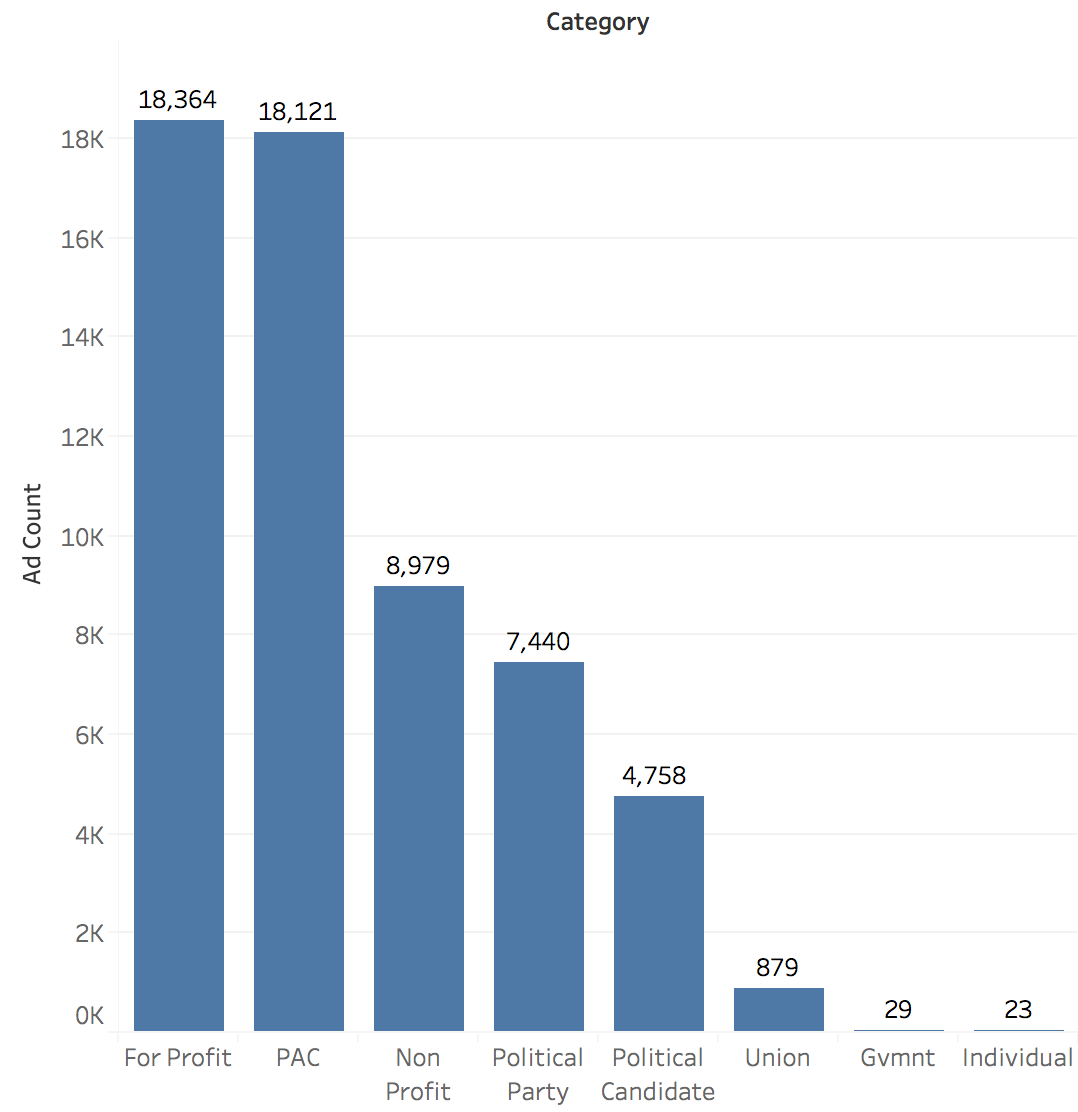
\includegraphics[width=0.8\textwidth]{ads_by_category.png}
    \captionof{figure}[width=0.4\textwidth]{Ads by Advertiser Category, Sept. 9\textsuperscript{th}, 2018 - Sept. 22\textsuperscript{nd}, 2018}
    \label{fig:ads_by_category}
\end{minipage}%
\begin{minipage}{.5\textwidth}

    \centering
    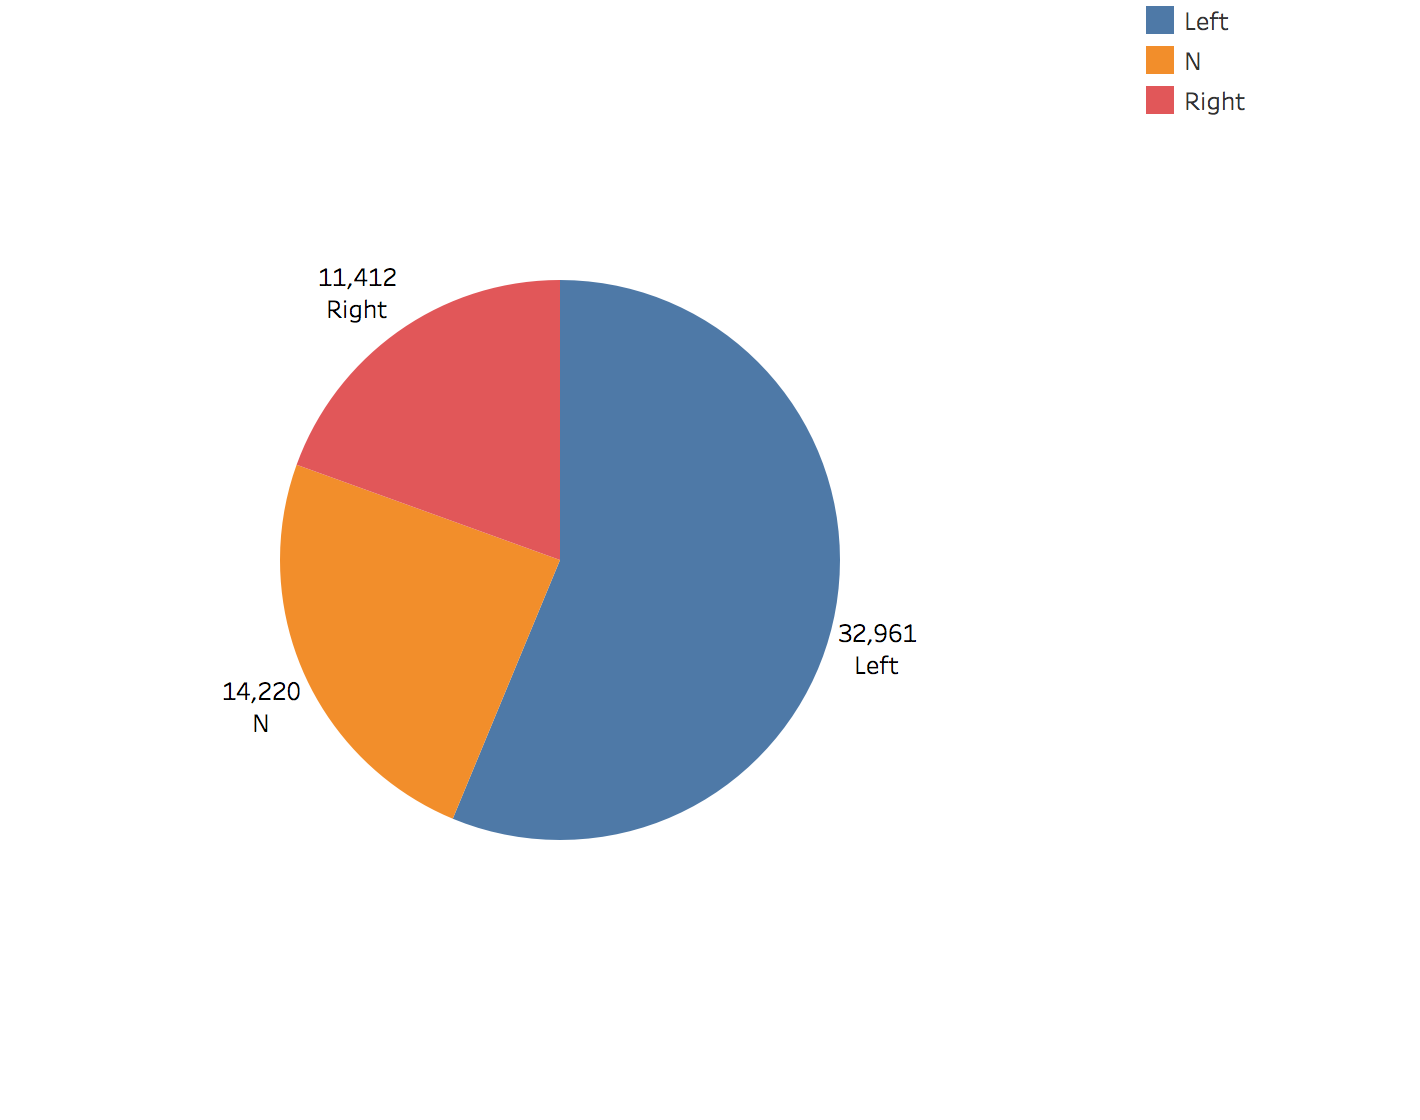
\includegraphics[width=1\textwidth]{ads_by_lean.png}
    \captionof{figure}{Ads by Partisan Lean, Sept. 9\textsuperscript{th}, 2018 - Sept. 22\textsuperscript{nd}, 2018}
    \label{fig:ads_by_lean}
\end{minipage}
\end{figure}

\begin{figure}
    \centering
    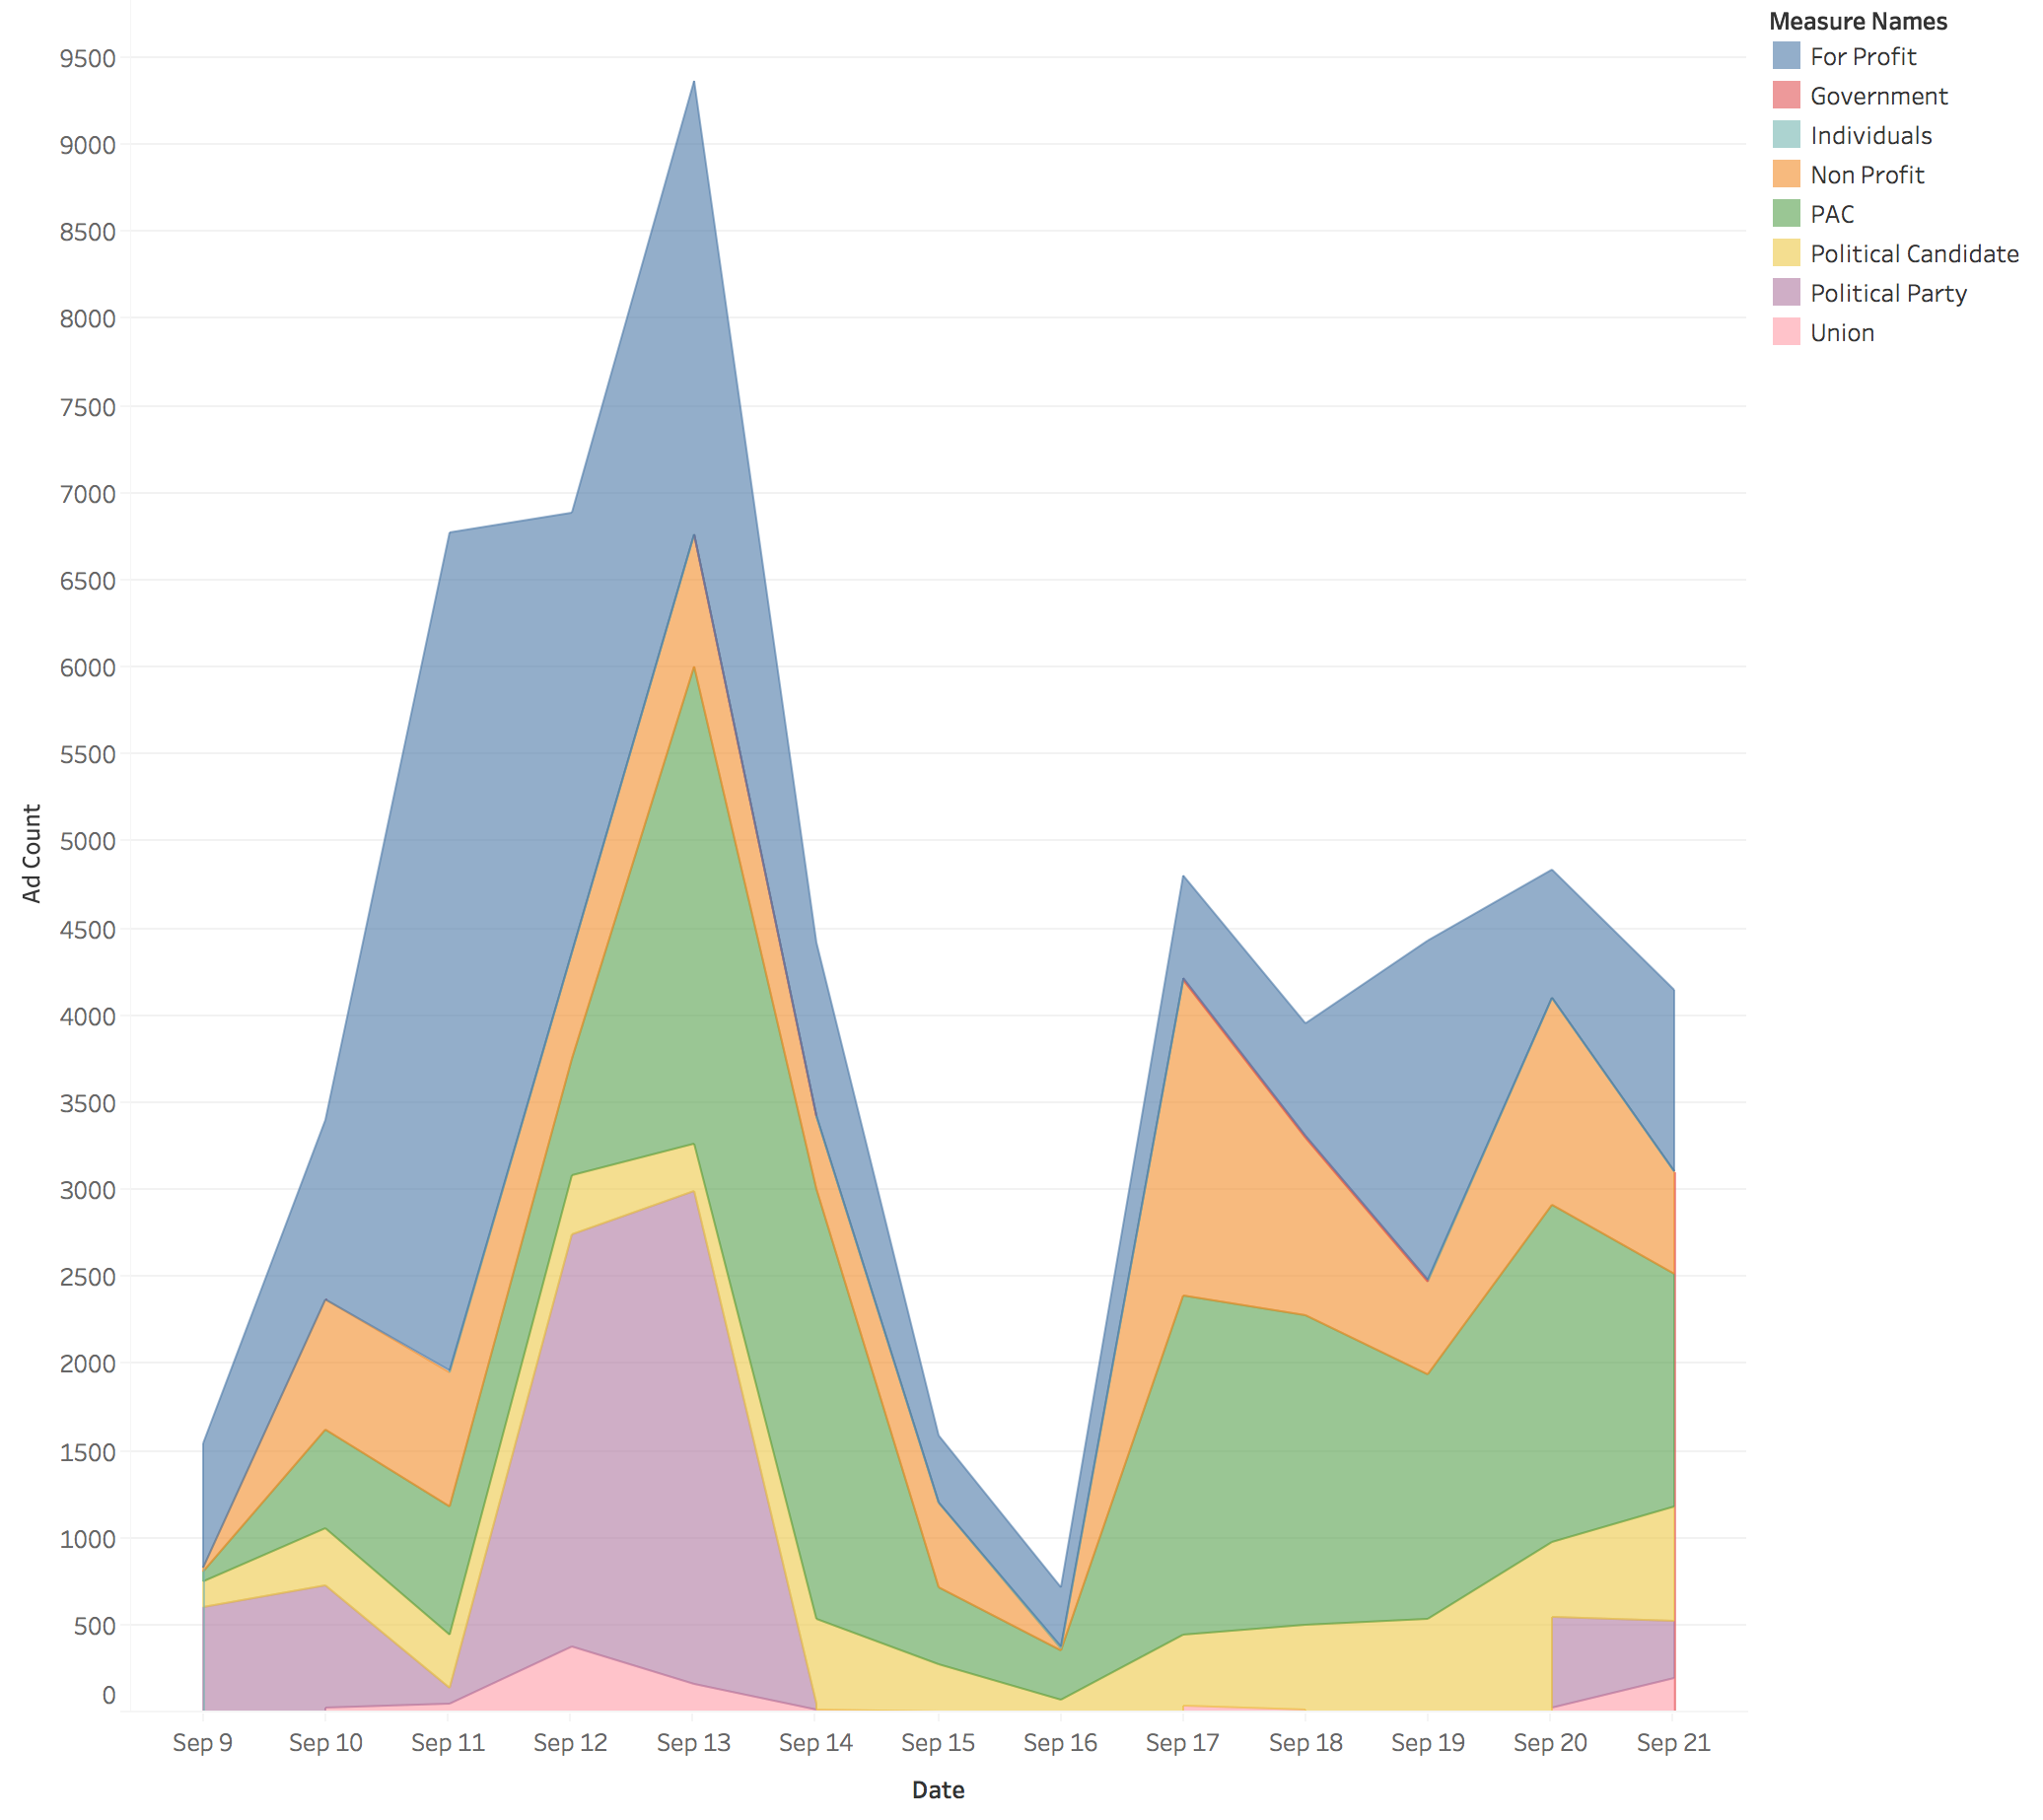
\includegraphics[width=0.6\textwidth]{categories_by_day.png}
    \caption{Daily Ads By Category}
    \label{fig:categories_by_day}
\end{figure}

\section*{Discussion}

\subsection*{Case Studies}

Here, we present a deep dive review of the online political advertising of two candidates and one PAC.

Beto O'Rourke is one of the few advertisers who is actively paying for ads on all three platforms. He is a Democratic candidate for Senate in Texas. During the time period of our study, September 9\textsuperscript{th} - September 22\textsuperscript{nd}, O'Rourke had 44 ads on Google properties with impressions, and spent \$ 213,500. 20 of those ads had fewer than 10,000 impressions, 13 had between 10,000 and 100,000 impressions, ten had 100,000 - 1 million impressions, and one had between one million and ten million impressions. These ads had total minimum impressions of LAE - write about geo targeting and keyword targeting after clarifying with Shawn. All these ads are AdWords text ads soliciting donations through ActBlue.com, a fundraising portal widely used by Democratic candidates. They would typically be shown to a user searching on google.com for a keyword targeted by the ad.
On Twitter, O'Rourke has 24 promoted tweets during the study period. These tweets are a mix of donation solicitations through actblue.com, awareness raising for events, and tweets aimed at generally increasing name recognition for the candidate. He spent \$58,265 on these tweets for a total of 3,756,650 impressions.
On Facebook, the Beto O'Rourke page had X ads, with a total spend of \$Y for a minimum of Z impressions. All these ads were paid for by "Beto for Texas", his campaign. Of these ads, x were between y and z impressions, x were between y and z impressions, etc.
Across the three platforms during the time period, Beto O'Rourke spent \$x for a total of at least x impressions. X\% of these impressions were on Facebook, Y\% of these impressions were on Google, and Z\% of these impressions were on Twitter. A notable fact about his advertising is that  all of the spending on the Beto O'Rourke Facebook page are paid for by the campaign itself, not PACs. This is not typical and we believe stems from the fact that the candidate has pledged not to accept any PAC money.
\begin{figure}
    \centering
    \centering
    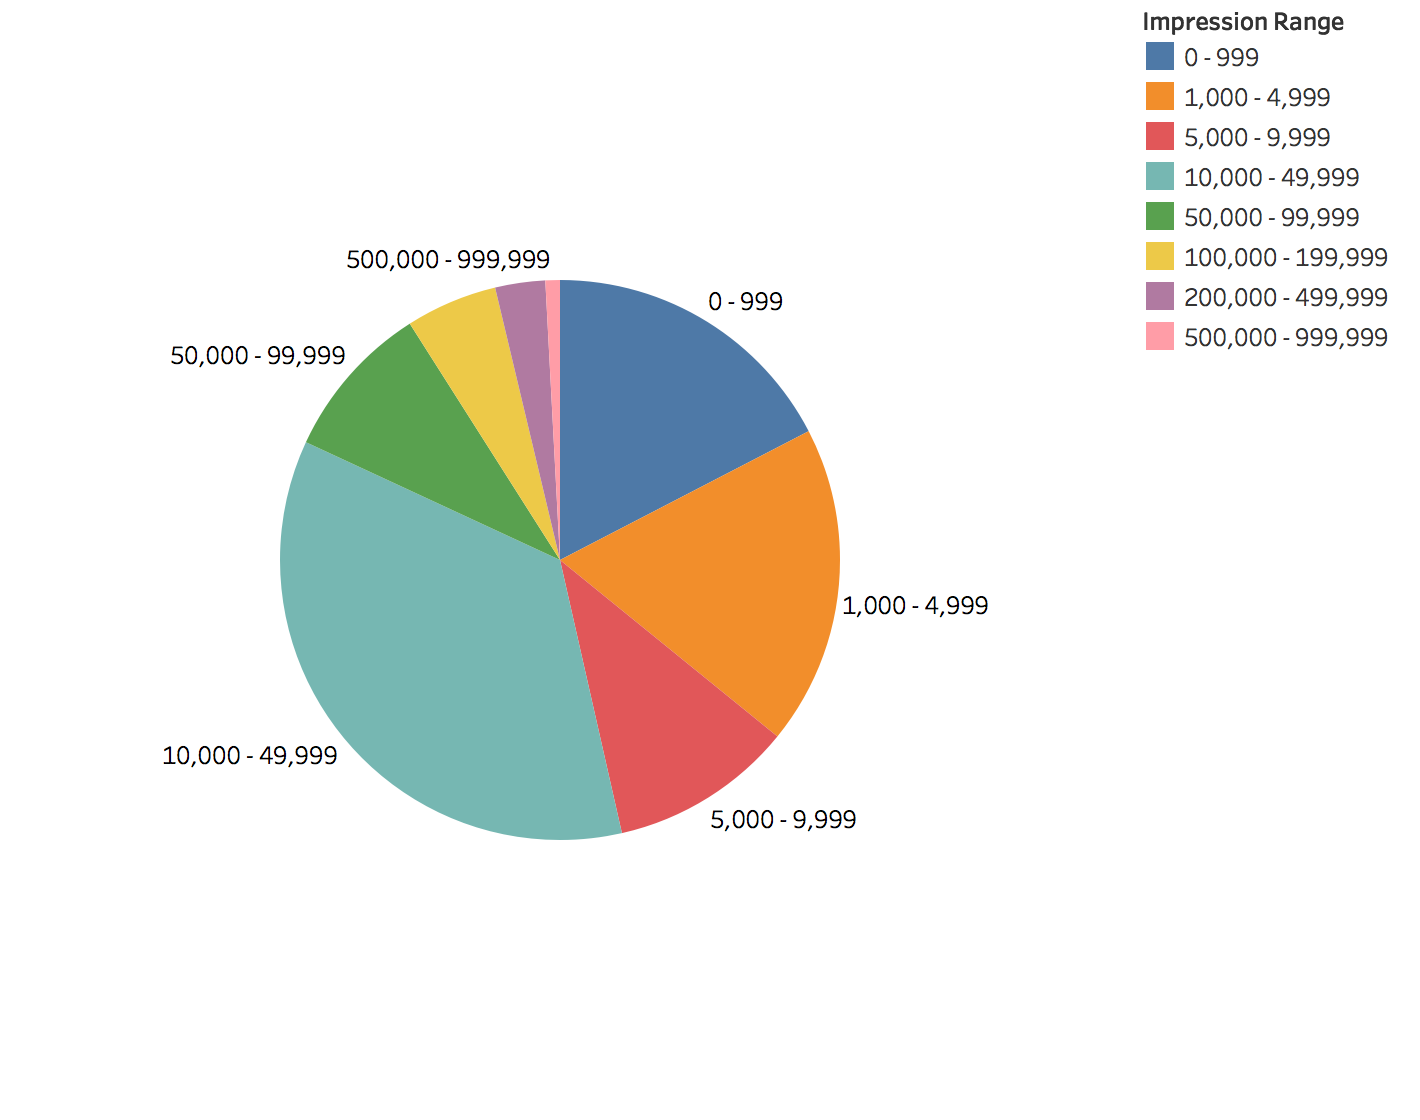
\includegraphics[width=0.5\textwidth]{beto_impression_pie.png}
    \caption{Distribution of Beto O'Rourke Ad by Impressions}
    \label{fig:beto_impression_pie}
\end{figure}
\begin{figure}
    \centering
    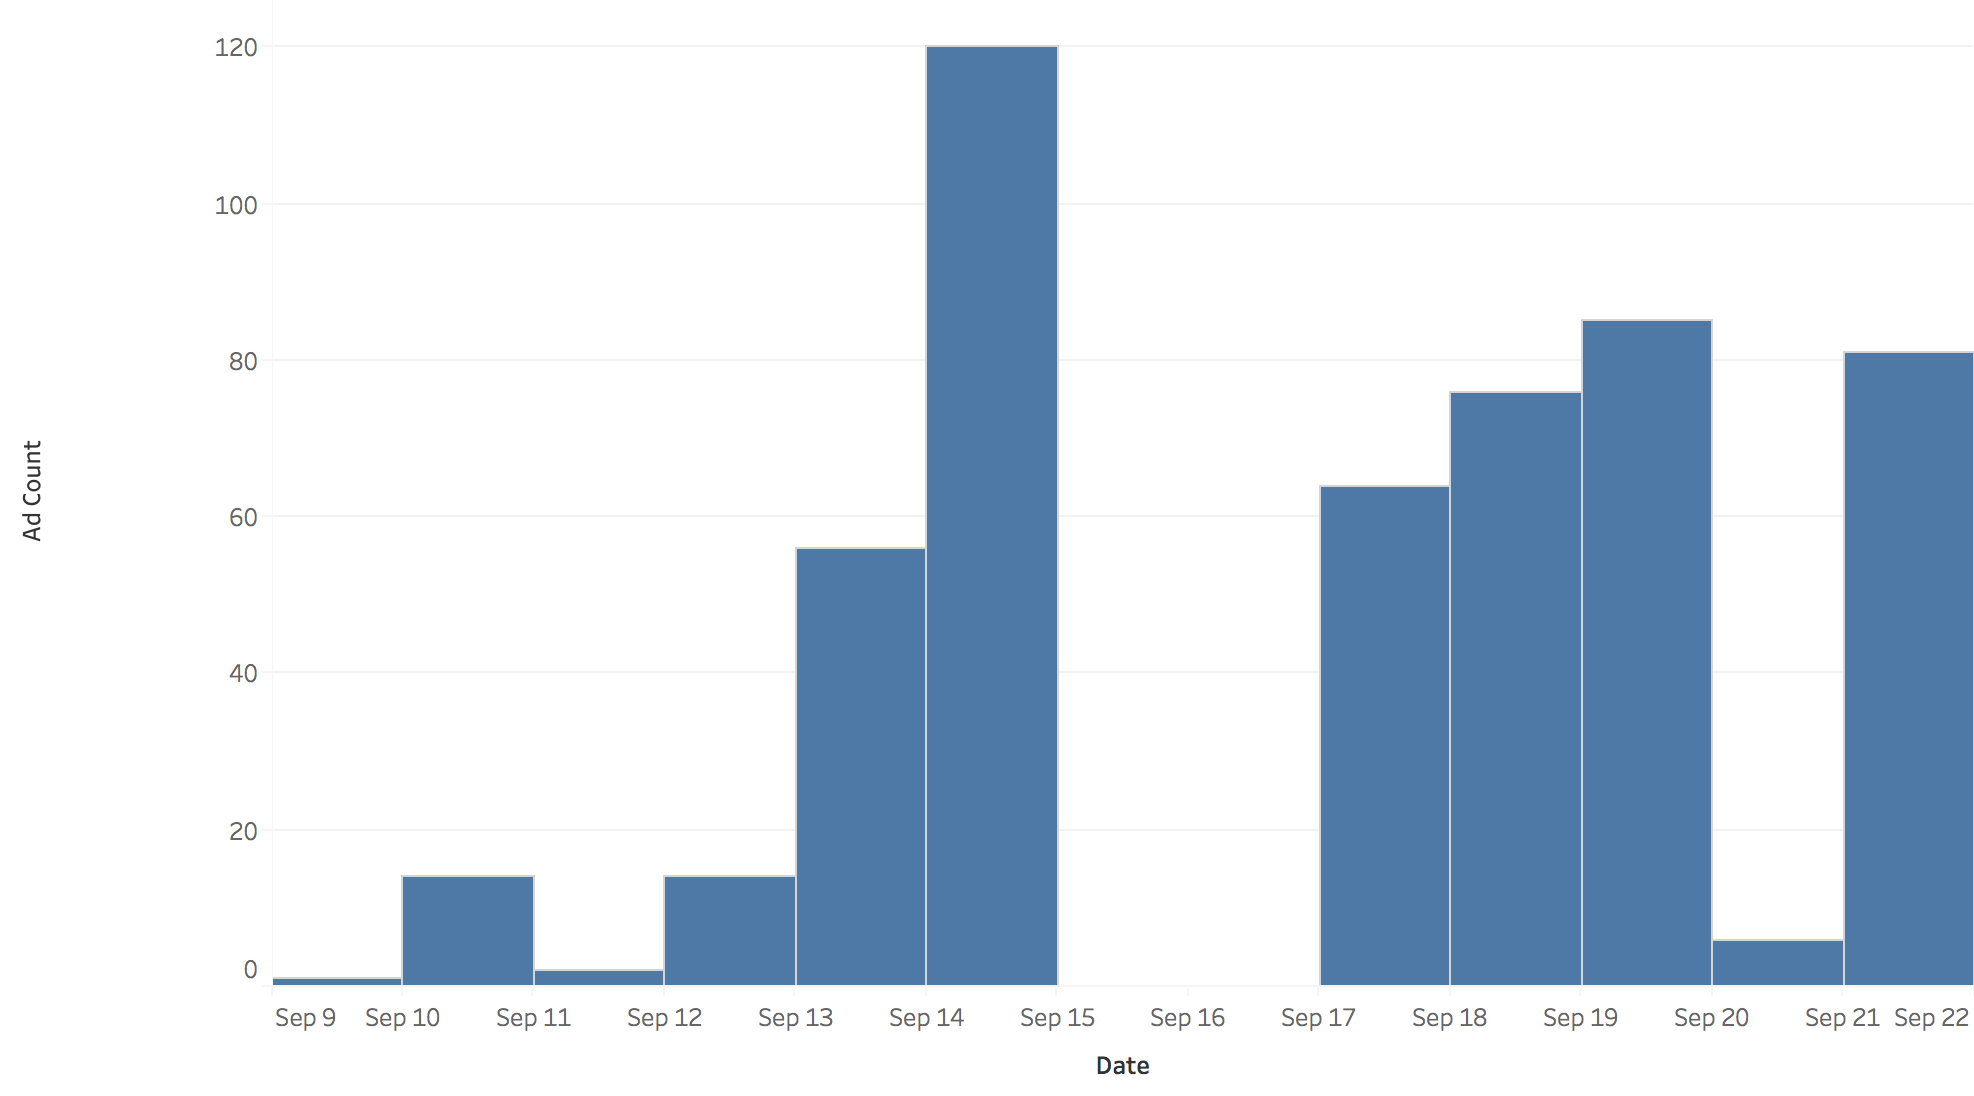
\includegraphics[width=0.5\textwidth]{beto_ads_by_day.png}
    \caption{Beto O'Rourke Daily Ad Count}
    \label{fig:beto_ads_by_day}
\end{figure}

Donald J. Trump is by far the most prolific political advertiser on Facebook. During the study period, we were able to find 7448 ads on his official page, but because of the rate limits described elsewhere in this paper, it's likely there were many ads we were not able to retrieve. Ads on this page are paid for by two different sponsors. Of the 7448, 4755 were paid for by "Donald J. Trump for President, Inc.", his campaign, and 2693 were paid for by "the Trump Make America Great Again Committee". He was much less active on Google during the study period. We were only able to find 27 ads during this time frame paid for by "the Trump Make America Great Again Committee" and none paid for by his campaign, although because these ads are relatively large, he was still the 12\textsuperscript{th} largest spender on the Google platform during the study period, with a total spend of \$13,1400 and total minimum impressions of 17,320,000. Donald Trump had no Promoted Tweets on Twitter, which we hypothesize because he has sufficient organic reach on that platform. 


\begin{figure}
\centering
\begin{minipage}{.5\textwidth}
  \centering
  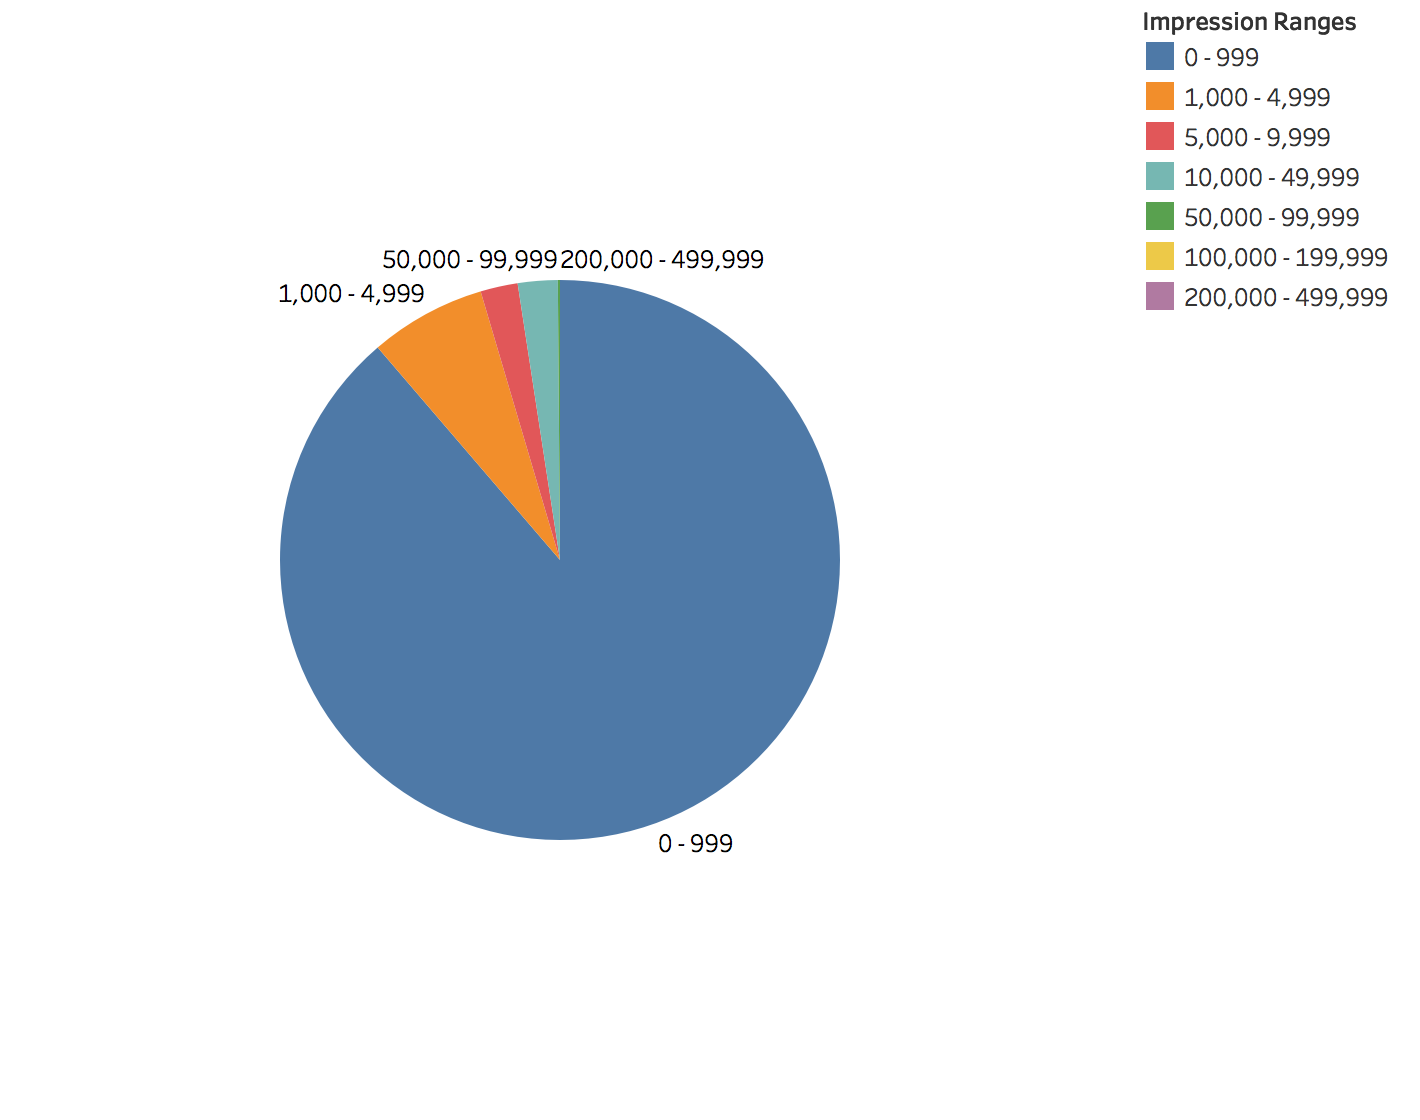
\includegraphics[width=.8\linewidth]{djt_campaign_impression_pie.png}
  \captionof{figure}{Donald J. Trump Campaign Ads by Impression Range}
  \label{fig:djt_impression_dist}
\end{minipage}%
\begin{minipage}{.5\textwidth}
  \centering
  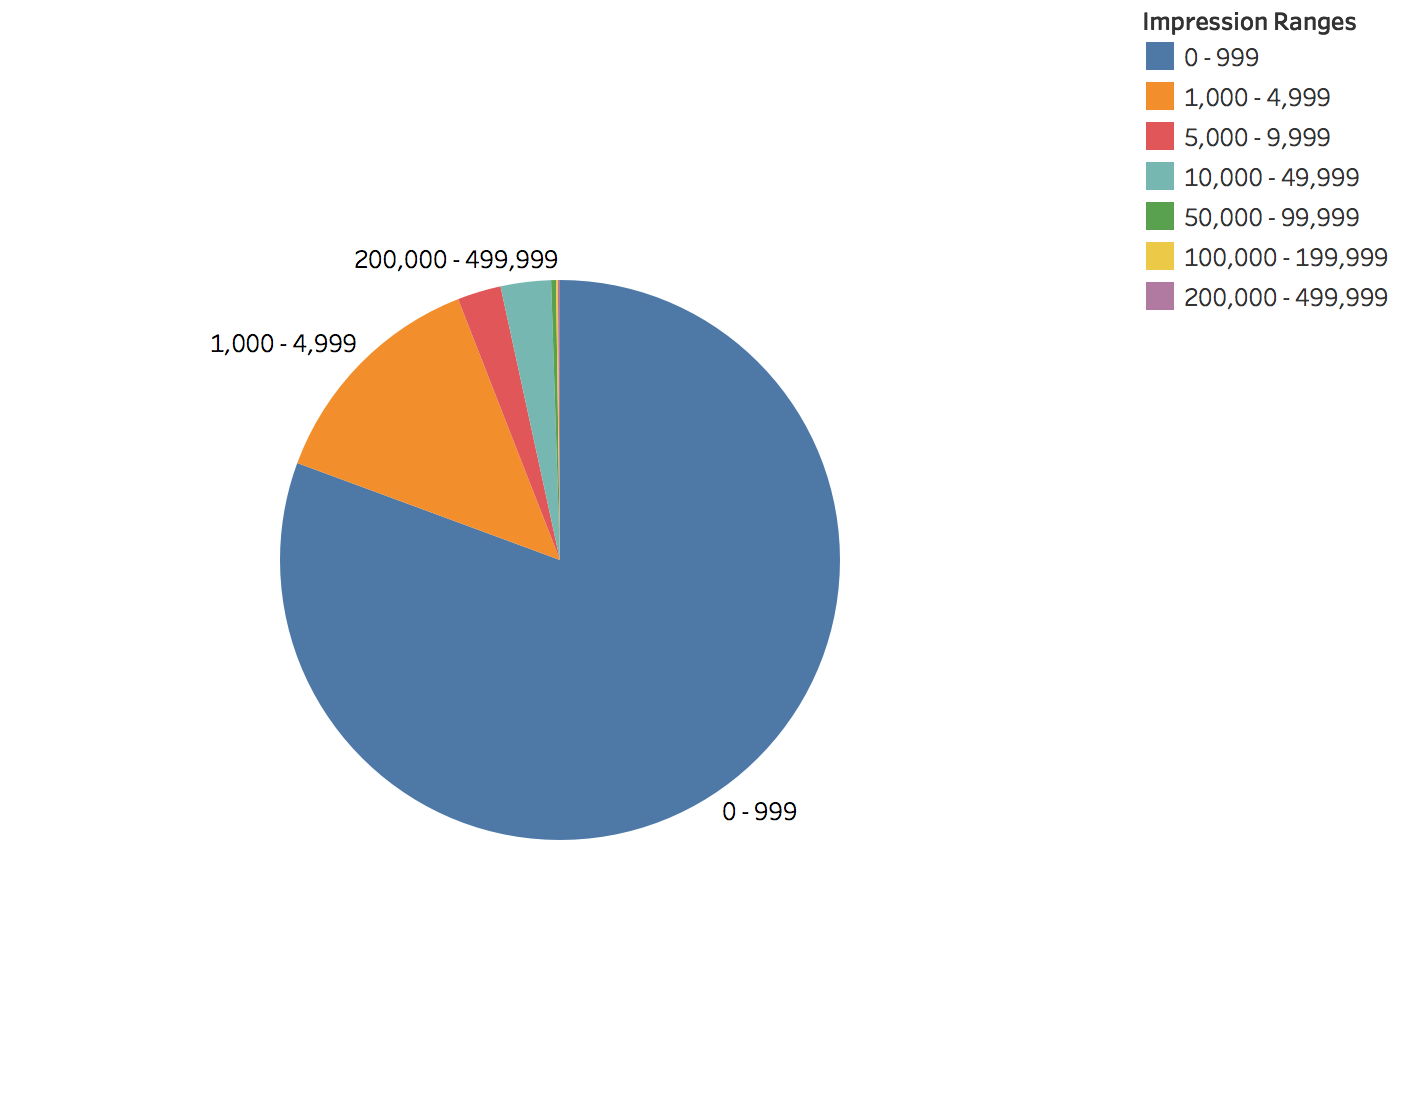
\includegraphics[width=.8\linewidth]{djt_maga_impression_pie.png}
  \captionof{figure}{Donald J. Trump MAGA Committee Ads by Impression Range}
  \label{fig:djt_maga_impression_dist}
\end{minipage}
\end{figure}

\begin{figure}
    \centering
    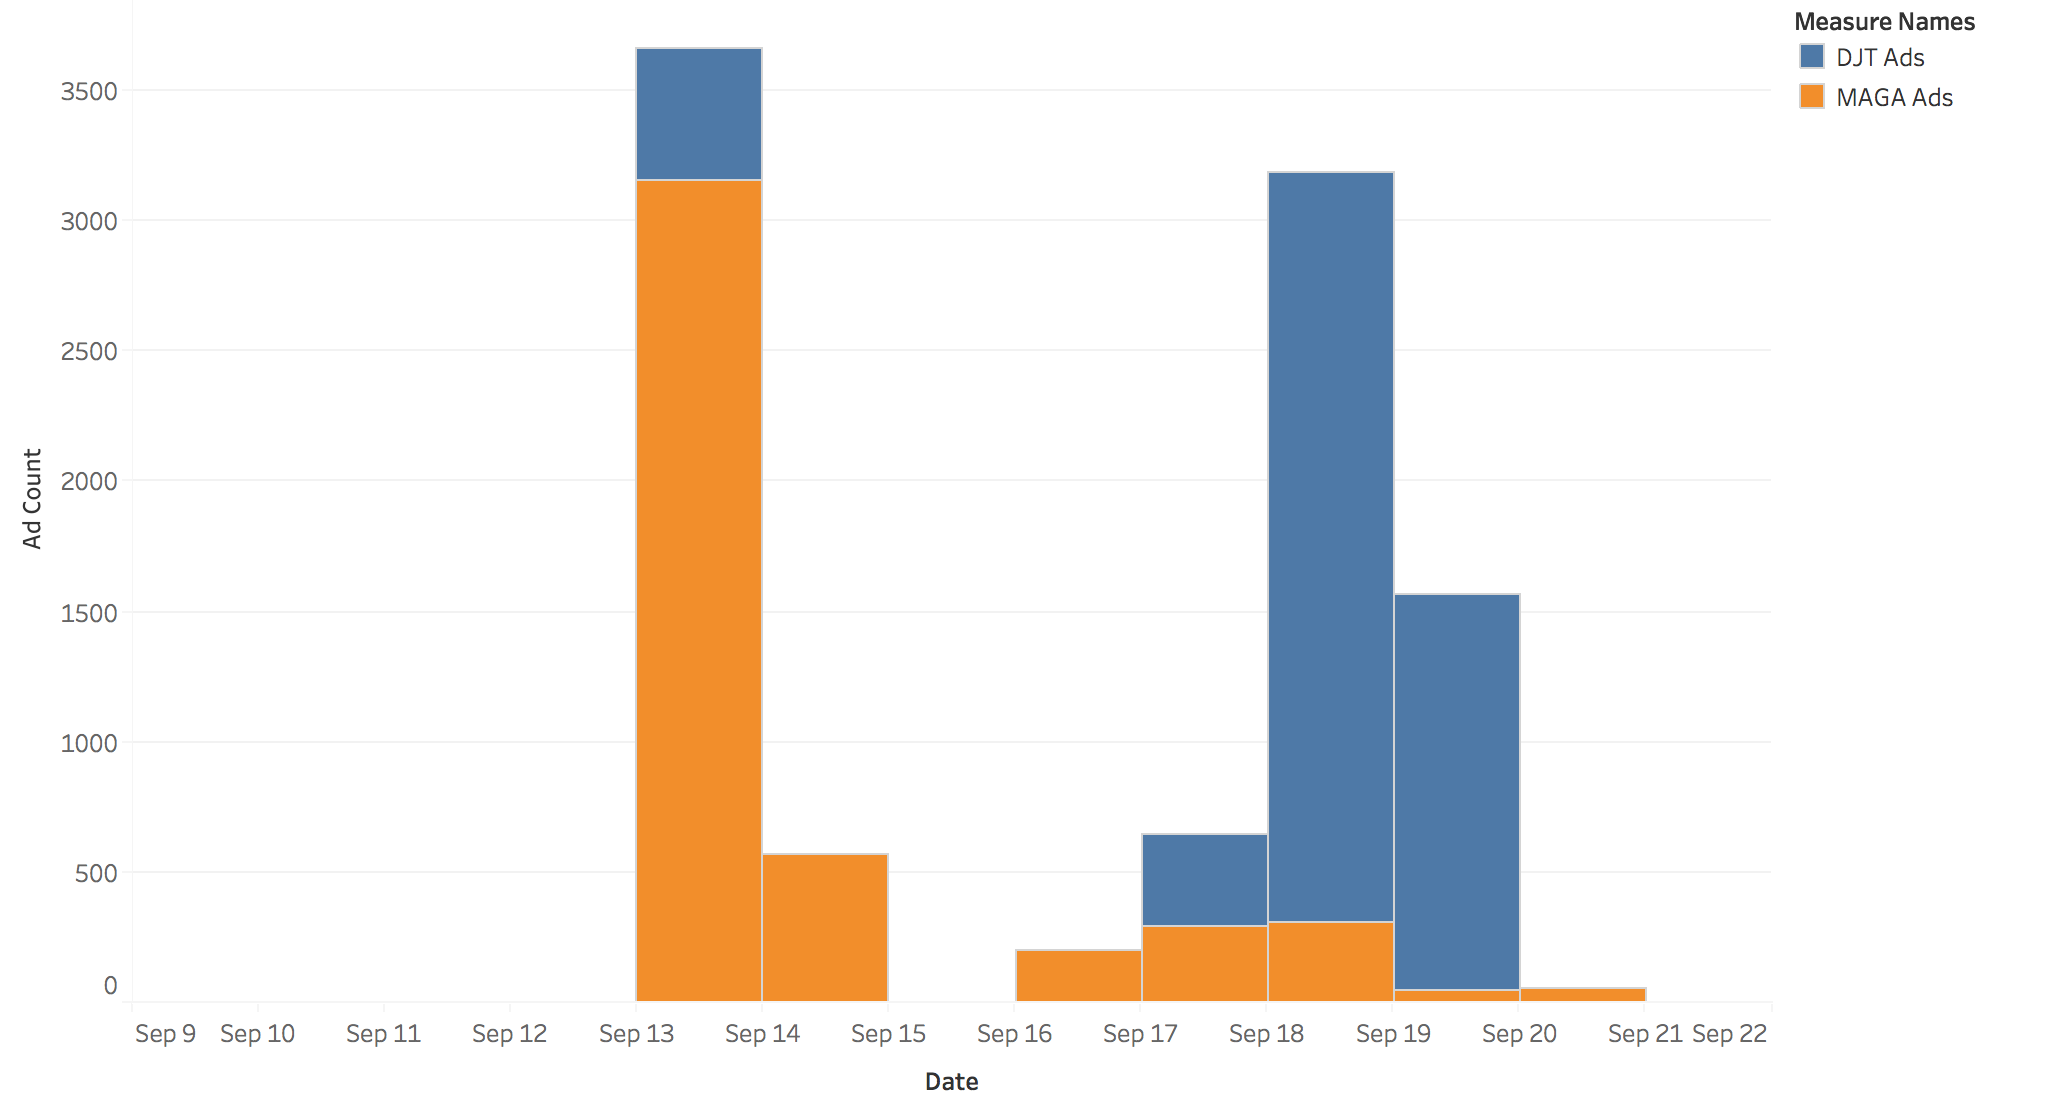
\includegraphics[width=.6\linewidth]{djt_ads_per_day.png}
    \caption{Donald J. Trump Page Ads per Day}
    \label{fig:djt_ads_per_day}
\end{figure}

\subsection*{Political Advertising Transparency Implementations}

Facebook, Google, and Twitter have all implemented their political advertising transparency efforts differently. Each of these political advertising transparency implementations has strengths and weaknesses with regards to what political advertisements are included, information released about sponsors and political advertisements, and this information is made accessible by third-parties. There is no ``best'' implementation rather each has some strengths and limitations that we will discuss in this subsection. We acknowledge that these transparency efforts have been quickly defined, implemented, deployed and all of the platforms are learning from feedback provided by different groups using their transparency archives and are likely working towards improving them.

Facebook is the most inclusive with respect to which advertisements it includes in their political advertisement. They include advertisements using three methods: 1) Advertisers can opt into including an advertisement in the transparency archive 2) Facebook has build a machine learning based system that flags advertisements as possibly political and they are then reviewed by human moderators 3) Facebook users can flag advertisements that they think are political but have not been labeled as political and these advertisements are then reviewed by human moderators. Facebook's inclusive policy has the drawback that some ads that are not directly politically related such as advertisements from a company selling solar panels is included in Facebook's political advertising transparency archive. This has created a backlash from companies that disagree with Facebook's definition of political advertising and feel their advertisements should not be made transparent and archived. The harm caused to a sponsor from potentially having their Facebook advertisements incorrectly labeled as political and included in the transparency archive seems minimal. From the perspective of someone analyzing the advertisements in Facebook's political archive, this inclusive policy is beneficial assuming that the different types of political advertisement can be categorized and those unrelated to a particular analysis can be ignored. Unless we have missed some substantial risk of harm to advertisers from making transparent and archiving their advertisements we advocate for a more inclusive policy similar to Facebook's.

Twitter and Google have a narrower policy with respect to the set of advertisements included in their political advertisement archives. Their policy currently focuses on including advertisements directly sponsored by U.S. federal election candidates and also advertisements related to these federal election candidates. Google and Twitter have also been less transparent about the methods they have deployed to select which advertisements and accounts are included in their political advertising transparency archives. Twitter has publicly announced that they plan to include political issue advertisement in the future and Google is also exploring how best to include a broader set of political advertisements. One drawback of the currently policies of all three platforms is that by only archiving political advertisements it is difficult to understand what if any political advertisements these platforms are missing and not making more transparent or archiving. Facebook does catch and add political ads to their transparency archive when they are found. We have also seen Twitter catch and add one federal election candidate's account to their transparency archive.

The next major difference between the transparency archive implementation is what information they make public about political sponsors and advertisements. Twitter make public the name and billing information for political advertisers which varies from the name and address of the advertising company to only a person's name. Google makes public the name of political advertisers and their Employer Identification Number (EIN) or Federal Election Candidate (FEC) ID number both of which can be linked to other public datasets to consistently and uniquely identify the advertiser. Facebook makes public a text string that should identify the sponsor and is provided by the advertiser. 

We have found that Facebook's method of identifying the sponsor leads to the most issues. The largest issue is that since sponsors often change the text string provided across different advertisements making it difficult to link ads from the same sponsor. Another lesser issue is that the text string is sometimes a cryptic acronym that is difficult to link to an organization or a name of a person instead of the organization. The current issues with sponsors' names likely introduced errors in our identification of sponsors and analysis based on sponsors. We have documented these issues in our reports and the steps we took to reduce this source of error. We hope that Facebook improves their handling of sponsors' names so that they will be more informative for people exposed to political content ads and ensure that future analysis will be more accurate.

The information made transparent by all platforms for each individual political advertisement includes the contents of the advertisement, an exact or range for amount spent, and exact or range for impressions. Twitter provides an exact amount spent and impression count rounded to the nearest hundred. Facebook and Google provide coarse-grained ranges provided for impressions and amount spent on each individual ad causes our analysis based on these ranges to be imprecise. We have tended to use the lower bound of these ranges so that our analysis based on these ranges should be thought of as a lower bound. Unfortunately, for Facebook many of the ads tend to be smaller ``micro-targeted'' ads where the lower bound might not be that meaningful given that they are in the \$0-\$99 USD range. The impression ranges are also problematic for micro-targeted ads given that they tend to generate between 0 - 1,000 or 1,001 - 5,000 impressions. We recommend that Facebook rethink these ranges especially for smaller quantities and offer finer-grained ranges. Micro-targeted ads are less prevalent on Google but the ranges provided by Google still cause error in our analysis. However, we understand the sensitivities that finer-grained ranges might expose information that impacts the competitiveness of Facebook and Google's advertising platforms. The other way of improving this is by releasing exact aggregate amount spent and impression information for all advertisements paid for by each sponsor which Google is currently providing but Facebook is not providing. This allows us and others to understand how much error is caused by the ranges provided and might enable researchers to estimate a more accurate number within the ranges provided instead of having to conservatively use the minimum. Additionally, we have found that all of the platforms periodically revise downwards the impression and spends. We assume this is caused by their fraud systems removing impressions and refunding the advertiser. This makes is difficult to exactly replicate results since the impressions and spend amounts are always slightly changing.

Facebook and Twitter are also providing demographics (i.e., gender, geolocation, and age ranges) information for the audiences that viewed each advertisement. Google is not providing audience demographic information but is providing keyword and geolocation targeting information. Twitter is also providing information about how political advertisements are targeted. Facebook is not providing information about how the targeted but some of the targeting can be inferred by the audience demographic information provided. It would be useful if Facebook also provided direct information about how an advertisement was targeted since our inferences about how an advertisement was targeted based on audience demographics might be incorrect.

Finally each of the three platforms have made their political advertising transparency data available using different methods of policies. Google has made their complete set of advertising transparency data available in a BigQuery (SQL-like) format which they update weekly and they have committed to keeping it public. Twitter has published a list of accounts that have promoted tweets included in their political archive. Twitter does not provide transparency information through their API but we have created a scraper which collects promoted tweets from these account that has so far not been blocked. We are publicly releasing the information that we have collected from scraping Twitter. Facebook has created a user portal where anyone with a Facebook account can search for ads with a set of keywords and view the results of their search by scrolling through 30 ads at a time. Currently is appears that Facebook's archive only allows someone to view the first 5,000 ads for a search it is unclear if this is a flaw in their user based archive portal of an intentional limit. Facebook has block our the scraper which we used to collected data from their portal for our prior analysis of political advertising on Facebook's platform. 

In August of 2018, Facebook granted a limited number of organizations in the U.S. (including our research group) access to an API which is still in beta testing. This API allows us to search Facebook's archive using keywords and collect data about political ads run on Facebook's platform at a larger scale. Currently Facebook's API has many limitations that cause us to have an incomplete set of data from their archive. The first is that using the API we can only retrieve the first 8,000 ads returned for a search. This means that it is currently challenging for us to collect data on many recent political ads. Another, significant limitation of Facebook's current API are rate limits in terms of number of queries and CPU usage. The combination of these limitations have made it effectively impossible to collect information about all of the political ads currently archived by Facebook using either the user portal or API. Finally, the agreement that we have signed with Facebook prevents us from publicly releasing the raw ad data that we collect using their API. 

Google's method of providing the political ad data they have made transparent in a well formatted database made their data the easiest for us to analyze and requires little additional work on our part to collate the missing ad text. Google has committed to making this dataset available to anyone. Twitter has provide their data in a way that requires us to create a custom scraper to collect it and another set of scripts to transform the scraped data and import it into our database. Twitter does not require someone to log into their platform and has not blocked our scrape. We have made the Twitter data that we have collected and the scripts for collecting and process it public. Facebook is currently the most limited of the three archives in terms of being able to access political ad information and publicly releasing it. Our analysis of Facebook's archive should be thought of as a lower bound since there are likely many ads and advertisers that we have missed. We hope that Facebook will improve access and transparency of political advertising on their platform.

Steps that Facebook could take are to increase or remove the query rate limits and accessible results per a query limitations from their API. The API could also be improved by allowing for date range searches along with keyword searches to enable easier data collection for groups with the goal of collecting all ads in their archive. It would also be useful if Facebook would allow raw ad data from their API to be shared publicly or provide a publicly accessible database version of all of the political ad information that they have archived. These improvements would bring the level of accessibility and transparency to on par with Google and Twitter's archives.

\bibliography{sample}

\section*{Acknowledgements}

\end{document}